
%% bare_conf.tex
%% V1.3
%% 2007/01/11
%% by Michael Shell
%% See:
%% http://www.michaelshell.org/
%% for current contact information.
%%
%% This is a skeleton file demonstrating the use of IEEEtran.cls
%% (requires IEEEtran.cls version 1.7 or later) with an IEEE conference paper.
%%
%% Support sites:
%% http://www.michaelshell.org/tex/ieeetran/
%% http://www.ctan.org/tex-archive/macros/latex/contrib/IEEEtran/
%% and
%% http://www.ieee.org/

%%*************************************************************************
%% Legal Notice:
%% This code is offered as-is without any warranty either expressed or
%% implied; without even the implied warranty of MERCHANTABILITY or
%% FITNESS FOR A PARTICULAR PURPOSE! 
%% User assumes all risk.
%% In no event shall IEEE or any contributor to this code be liable for
%% any damages or losses, including, but not limited to, incidental,
%% consequential, or any other damages, resulting from the use or misuse
%% of any information contained here.
%%
%% All comments are the opinions of their respective authors and are not
%% necessarily endorsed by the IEEE.
%%
%% This work is distributed under the LaTeX Project Public License (LPPL)
%% ( http://www.latex-project.org/ ) version 1.3, and may be freely used,
%% distributed and modified. A copy of the LPPL, version 1.3, is included
%% in the base LaTeX documentation of all distributions of LaTeX released
%% 2003/12/01 or later.
%% Retain all contribution notices and credits.
%% ** Modified files should be clearly indicated as such, including  **
%% ** renaming them and changing author support contact information. **
%%
%% File list of work: IEEEtran.cls, IEEEtran_HOWTO.pdf, bare_adv.tex,
%%                    bare_conf.tex, bare_jrnl.tex, bare_jrnl_compsoc.tex
%%*************************************************************************

% *** Authors should verify (and, if needed, correct) their LaTeX system  ***
% *** with the testflow diagnostic prior to trusting their LaTeX platform ***
% *** with production work. IEEE's font choices can trigger bugs that do  ***
% *** not appear when using other class files.                            ***
% The testflow support page is at:
% http://www.michaelshell.org/tex/testflow/



% Note that the a4paper option is mainly intended so that authors in
% countries using A4 can easily print to A4 and see how their papers will
% look in print - the typesetting of the document will not typically be
% affected with changes in paper size (but the bottom and side margins will).
% Use the testflow package mentioned above to verify correct handling of
% both paper sizes by the user's LaTeX system.
%
% Also note that the "draftcls" or "draftclsnofoot", not "draft", option
% should be used if it is desired that the figures are to be displayed in
% draft mode.
%
\documentclass[conference]{IEEEtran}
\usepackage{blindtext, graphicx}
% Add the compsoc option for Computer Society conferences.
%
% If IEEEtran.cls has not been installed into the LaTeX system files,
% manually specify the path to it like:
% \documentclass[conference]{../sty/IEEEtran}
% Some very useful LaTeX packages include:
% (uncomment the ones you want to load)


% *** MISC UTILITY PACKAGES ***
%
%\usepackage{ifpdf}
% Heiko Oberdiek's ifpdf.sty is very useful if you need conditional
% compilation based on whether the output is pdf or dvi.
% usage:
% \ifpdf
%   % pdf code
% \else
%   % dvi code
% \fi
% The latest version of ifpdf.sty can be obtained from:
% http://www.ctan.org/tex-archive/macros/latex/contrib/oberdiek/
% Also, note that IEEEtran.cls V1.7 and later provides a builtin
% \ifCLASSINFOpdf conditional that works the same way.
% When switching from latex to pdflatex and vice-versa, the compiler may
% have to be run twice to clear warning/error messages.






% *** CITATION PACKAGES ***
%
%\usepackage{cite}
% cite.sty was written by Donald Arseneau
% V1.6 and later of IEEEtran pre-defines the format of the cite.sty package
% \cite{} output to follow that of IEEE. Loading the cite package will
% result in citation numbers being automatically sorted and properly
% "compressed/ranged". e.g., [1], [9], [2], [7], [5], [6] without using
% cite.sty will become [1], [2], [5]--[7], [9] using cite.sty. cite.sty's
% \cite will automatically add leading space, if needed. Use cite.sty's
% noadjust option (cite.sty V3.8 and later) if you want to turn this off.
% cite.sty is already installed on most LaTeX systems. Be sure and use
% version 4.0 (2003-05-27) and later if using hyperref.sty. cite.sty does
% not currently provide for hyperlinked citations.
% The latest version can be obtained at:
% http://www.ctan.org/tex-archive/macros/latex/contrib/cite/
% The documentation is contained in the cite.sty file itself.






% *** GRAPHICS RELATED PACKAGES ***
%
\ifCLASSINFOpdf
  % \usepackage[pdftex]{graphicx}
  % declare the path(s) where your graphic files are
  % \graphicspath{{../pdf/}{../jpeg/}}
  % and their extensions so you won't have to specify these with
  % every instance of \includegraphics
  % \DeclareGraphicsExtensions{.pdf,.jpeg,.png}
\else
  % or other class option (dvipsone, dvipdf, if not using dvips). graphicx
  % will default to the driver specified in the system graphics.cfg if no
  % driver is specified.
  % \usepackage[dvips]{graphicx}
  % declare the path(s) where your graphic files are
  % \graphicspath{{../eps/}}
  % and their extensions so you won't have to specify these with
  % every instance of \includegraphics
  % \DeclareGraphicsExtensions{.eps}
\fi
% graphicx was written by David Carlisle and Sebastian Rahtz. It is
% required if you want graphics, photos, etc. graphicx.sty is already
% installed on most LaTeX systems. The latest version and documentation can
% be obtained at: 
% http://www.ctan.org/tex-archive/macros/latex/required/graphics/
% Another good source of documentation is "Using Imported Graphics in
% LaTeX2e" by Keith Reckdahl which can be found as epslatex.ps or
% epslatex.pdf at: http://www.ctan.org/tex-archive/info/
%
% latex, and pdflatex in dvi mode, support graphics in encapsulated
% postscript (.eps) format. pdflatex in pdf mode supports graphics
% in .pdf, .jpeg, .png and .mps (metapost) formats. Users should ensure
% that all non-photo figures use a vector format (.eps, .pdf, .mps) and
% not a bitmapped formats (.jpeg, .png). IEEE frowns on bitmapped formats
% which can result in "jaggedy"/blurry rendering of lines and letters as
% well as large increases in file sizes.
%
% You can find documentation about the pdfTeX application at:
% http://www.tug.org/applications/pdftex





% *** MATH PACKAGES ***
%
%\usepackage[cmex10]{amsmath}
% A popular package from the American Mathematical Society that provides
% many useful and powerful commands for dealing with mathematics. If using
% it, be sure to load this package with the cmex10 option to ensure that
% only type 1 fonts will utilized at all point sizes. Without this option,
% it is possible that some math symbols, particularly those within
% footnotes, will be rendered in bitmap form which will result in a
% document that can not be IEEE Xplore compliant!
%
% Also, note that the amsmath package sets \interdisplaylinepenalty to 10000
% thus preventing page breaks from occurring within multiline equations. Use:
%\interdisplaylinepenalty=2500
% after loading amsmath to restore such page breaks as IEEEtran.cls normally
% does. amsmath.sty is already installed on most LaTeX systems. The latest
% version and documentation can be obtained at:
% http://www.ctan.org/tex-archive/macros/latex/required/amslatex/math/





% *** SPECIALIZED LIST PACKAGES ***
%
%\usepackage{algorithmic}
% algorithmic.sty was written by Peter Williams and Rogerio Brito.
% This package provides an algorithmic environment fo describing algorithms.
% You can use the algorithmic environment in-text or within a figure
% environment to provide for a floating algorithm. Do NOT use the algorithm
% floating environment provided by algorithm.sty (by the same authors) or
% algorithm2e.sty (by Christophe Fiorio) as IEEE does not use dedicated
% algorithm float types and packages that provide these will not provide
% correct IEEE style captions. The latest version and documentation of
% algorithmic.sty can be obtained at:
% http://www.ctan.org/tex-archive/macros/latex/contrib/algorithms/
% There is also a support site at:
% http://algorithms.berlios.de/index.html
% Also of interest may be the (relatively newer and more customizable)
% algorithmicx.sty package by Szasz Janos:
% http://www.ctan.org/tex-archive/macros/latex/contrib/algorithmicx/




% *** ALIGNMENT PACKAGES ***
%
%\usepackage{array}
% Frank Mittelbach's and David Carlisle's array.sty patches and improves
% the standard LaTeX2e array and tabular environments to provide better
% appearance and additional user controls. As the default LaTeX2e table
% generation code is lacking to the point of almost being broken with
% respect to the quality of the end results, all users are strongly
% advised to use an enhanced (at the very least that provided by array.sty)
% set of table tools. array.sty is already installed on most systems. The
% latest version and documentation can be obtained at:
% http://www.ctan.org/tex-archive/macros/latex/required/tools/


%\usepackage{mdwmath}
%\usepackage{mdwtab}
% Also highly recommended is Mark Wooding's extremely powerful MDW tools,
% especially mdwmath.sty and mdwtab.sty which are used to format equations
% and tables, respectively. The MDWtools set is already installed on most
% LaTeX systems. The lastest version and documentation is available at:
% http://www.ctan.org/tex-archive/macros/latex/contrib/mdwtools/


% IEEEtran contains the IEEEeqnarray family of commands that can be used to
% generate multiline equations as well as matrices, tables, etc., of high
% quality.


%\usepackage{eqparbox}
% Also of notable interest is Scott Pakin's eqparbox package for creating
% (automatically sized) equal width boxes - aka "natural width parboxes".
% Available at:
% http://www.ctan.org/tex-archive/macros/latex/contrib/eqparbox/





% *** SUBFIGURE PACKAGES ***
%\usepackage[tight,footnotesize]{subfigure}
% subfigure.sty was written by Steven Douglas Cochran. This package makes it
% easy to put subfigures in your figures. e.g., "Figure 1a and 1b". For IEEE
% work, it is a good idea to load it with the tight package option to reduce
% the amount of white space around the subfigures. subfigure.sty is already
% installed on most LaTeX systems. The latest version and documentation can
% be obtained at:
% http://www.ctan.org/tex-archive/obsolete/macros/latex/contrib/subfigure/
% subfigure.sty has been superceeded by subfig.sty.



%\usepackage[caption=false]{caption}
%\usepackage[font=footnotesize]{subfig}
% subfig.sty, also written by Steven Douglas Cochran, is the modern
% replacement for subfigure.sty. However, subfig.sty requires and
% automatically loads Axel Sommerfeldt's caption.sty which will override
% IEEEtran.cls handling of captions and this will result in nonIEEE style
% figure/table captions. To prevent this problem, be sure and preload
% caption.sty with its "caption=false" package option. This is will preserve
% IEEEtran.cls handing of captions. Version 1.3 (2005/06/28) and later 
% (recommended due to many improvements over 1.2) of subfig.sty supports
% the caption=false option directly:
%\usepackage[caption=false,font=footnotesize]{subfig}
%
% The latest version and documentation can be obtained at:
% http://www.ctan.org/tex-archive/macros/latex/contrib/subfig/
% The latest version and documentation of caption.sty can be obtained at:
% http://www.ctan.org/tex-archive/macros/latex/contrib/caption/




% *** FLOAT PACKAGES ***
%
%\usepackage{fixltx2e}
% fixltx2e, the successor to the earlier fix2col.sty, was written by
% Frank Mittelbach and David Carlisle. This package corrects a few problems
% in the LaTeX2e kernel, the most notable of which is that in current
% LaTeX2e releases, the ordering of single and double column floats is not
% guaranteed to be preserved. Thus, an unpatched LaTeX2e can allow a
% single column figure to be placed prior to an earlier double column
% figure. The latest version and documentation can be found at:
% http://www.ctan.org/tex-archive/macros/latex/base/



%\usepackage{stfloats}
% stfloats.sty was written by Sigitas Tolusis. This package gives LaTeX2e
% the ability to do double column floats at the bottom of the page as well
% as the top. (e.g., "\begin{figure*}[!b]" is not normally possible in
% LaTeX2e). It also provides a command:
%\fnbelowfloat
% to enable the placement of footnotes below bottom floats (the standard
% LaTeX2e kernel puts them above bottom floats). This is an invasive package
% which rewrites many portions of the LaTeX2e float routines. It may not work
% with other packages that modify the LaTeX2e float routines. The latest
% version and documentation can be obtained at:
% http://www.ctan.org/tex-archive/macros/latex/contrib/sttools/
% Documentation is contained in the stfloats.sty comments as well as in the
% presfull.pdf file. Do not use the stfloats baselinefloat ability as IEEE
% does not allow \baselineskip to stretch. Authors submitting work to the
% IEEE should note that IEEE rarely uses double column equations and
% that authors should try to avoid such use. Do not be tempted to use the
% cuted.sty or midfloat.sty packages (also by Sigitas Tolusis) as IEEE does
% not format its papers in such ways.


% *** PDF, URL AND HYPERLINK PACKAGES ***
%
%\usepackage{url}
% url.sty was written by Donald Arseneau. It provides better support for
% handling and breaking URLs. url.sty is already installed on most LaTeX
% systems. The latest version can be obtained at:
% http://www.ctan.org/tex-archive/macros/latex/contrib/misc/
% Read the url.sty source comments for usage information. Basically,
% \url{my_url_here}.





% *** Do not adjust lengths that control margins, column widths, etc. ***
% *** Do not use packages that alter fonts (such as pslatex).         ***
% There should be no need to do such things with IEEEtran.cls V1.6 and later.
% (Unless specifically asked to do so by the journal or conference you plan
% to submit to, of course. )


% correct bad hyphenation here
\usepackage[english]{babel} % English language/hyphenation
\usepackage{array}
\usepackage{multirow}
\usepackage{amsmath}
\numberwithin{equation}{section}
\numberwithin{figure}{section}
\numberwithin{table}{section}
\usepackage{caption}
\usepackage{listings}
\usepackage{color}
 
\definecolor{codegreen}{rgb}{0,0.6,0}
\definecolor{codegray}{rgb}{0.5,0.5,0.5}
\definecolor{codepurple}{rgb}{0.58,0,0.82}
\definecolor{backcolour}{rgb}{0.95,0.95,0.92}
 
\lstdefinestyle{mystyle}{
    backgroundcolor=\color{backcolour},
    commentstyle=\color{codegreen},
    keywordstyle=\color{magenta},
    numberstyle=\tiny\color{codegray},
    stringstyle=\color{codepurple},
    basicstyle=\footnotesize,
    breakatwhitespace=false,         
    breaklines=true,                 
    captionpos=b,                    
    keepspaces=true,                 
    numbers=left,                    
    numbersep=5pt,                  
    showspaces=false,                
    showstringspaces=false,
    showtabs=false,                  
    tabsize=2
}
\lstset{style=mystyle}
\begin{document}

%
% paper title
% can use linebreaks \\ within to get better formatting as desired
\title{A Comparative study of different Machine Learning techniques on Kaggle Twitter Social Influencers Data Set}
\author{\IEEEauthorblockN{Arora, Pragya\IEEEauthorrefmark{1},
Ghai, Piyush\IEEEauthorrefmark{2}, Gupta, Harsh\IEEEauthorrefmark{3} and
Ramkrishnan, Navnith\IEEEauthorrefmark{4}}
\IEEEauthorblockA{Department of Computer Science \& Engineering,
The Ohio State University\\
Columbus, OH 43202\\
Email: \IEEEauthorrefmark{1}arora.170@osu.edu,
\IEEEauthorrefmark{2}ghai.8@osu.edu,
\IEEEauthorrefmark{3}gupta.749@osu.edu,
\IEEEauthorrefmark{4}ramkrishnan.1@osu.edu}}
\maketitle


\begin{abstract}
%\boldmath
Social media like twitter has given advent to growing importance to understand the behavior of these networks. More importantly these graph networks shows different patterns which are interesting to analyze. Some nodes becomes almost a sink where as some node acts like a source of outgoing links. Understanding these patterns will help in various applications and specially in experiments like Network A/B Testing where we need to introduce some new features to a treatment group restricting the control group. In out project we intended to experiment and analyze on one such pattern where we try to identify which node is more influential when compared to another node. To understand such a behavior we used a Twitter network data set which had 11 features for each node and we applied machine learning techniques to understanding the underlying features to classify the task at hand.
 
\end{abstract}
% IEEEtran.cls defaults to using nonbold math in the Abstract.
% This preserves the distinction between vectors and scalars. However,
% if the journal you are submitting to favors bold math in the abstract,
% then you can use LaTeX's standard command \boldmath at the very start
% of the abstract to achieve this. Many IEEE journals frown on math
% in the abstract anyway.

% Note that keywords are not normally used for peerreview papers.
\section{Introduction}
The growing importance of Social Networks has given an impetus to understand more about its implications because networks like these can influence millions of people. Contrary to paper or television media, social media is far more reaching to the audiences across the world and information exchange has never seen such a revolution. The need of the time is to have an The ability to understand the nuances of these networks because with more connectivity it becomes crucial to understand the behavior of different nodes in the network.

Some nodes/users are more important than others as there behavior affects a larger sets of nodes in the graph. When a user of such a graph is using the network she/he may find some activity shared by some of the other nodes more striking than others. A lot of psychological and cognitive science study shows that ones life is greatly impacted by her/his immediately surrounding and their influence. As social network has become a part of everyone's life, it has become important which are the nodes which has more impact on others i.e which are influential. One application of such a study is to predict what is the general mood of the crowd during election by analyzing the social network handle of all the candidates who stood for it. 

In this project, we address a targeted challenge of this problem presented in a Kaggle\cite{kaggle} competition from 2013 , in which influencers on Twitter is predicted from a set of features derived from user activity on the network, such as follower count, retweets received, etc. Rather than identifying influencers in the larger network, we are asked to simply identify which of a pair of users, A and B, is more influential, based on information about their respective activity in the network. This is a binary-classification problem. To find an optimal prediction method, we applied pre-processing methods including feature transformations and dimensionality reduction via principal component analysis (PCA). We used four different machinelearning algorithms—Logistic Regression, Support Vector Machines (SVM), Neural Network, and Gradient Boosting—to model the data. We also tried varying some of the decision boundary options for the SVM by using different kernels and neural network classifiers by varying the activation functions on the hidden layer. Our approach includes a few methods that we did not see in other attempts at this problem, specifically a logarithmic feature transformation, the application of feature selection and gradient boosting. Outside of gradient boosting, the model configurations which produced the best results used linear-like decision boundaries (Logistic Regression).
 
\section{DATASET}\label{sec:page-layout}

This section expands on the data set which we used to try the different models on. 


\subsection{Original Dataset}\label{sec:formatting}
The data set which we used came from a Kaggle contest. The data set had a 
\begin{itemize}
  \item train.csv
  \item test.csv
  \item sample\_predicitions.csv
\end{itemize}

The train.csv file contains data points where each data point is a pair wise features for two users along with a binary value which reflects which user is more influential. If the value is 0 the first user is more influential and vice-verse. Each user has 11 unique features which are extracted from their twitter profile and recorded in numeric form. The 11 features extracted includes:

\begin{itemize}
  \item Follwers
  \item Follwing
  \item Listed
  \item Mentions received
  \item Re-tweets received
  \item Mentions sent
  \item Re-tweets sent
  \item Posts
  \item Network Feature 1
  \item Network Feature 2
  \item Network Feature 2
\end{itemize}

Similarly we have features for two users in each data item in the testing file but the testing file has no class label. There are 5500 training samples and 5953 testing samples in our data set. Given a test sample, our job is to predict which individual in this test sample is more influential.

\subsection{Kaggle Competition}
The Kaggle competition is hosted at : \cite{kaggle2}. The evaluation for this competition is based on area under the ROC curve. \cite{roc}.

\subsection{Data Preprocessing
}\label{sec:formatting-text}

Since the data is a numerical data, we use some pre-processing techniques on it. The dataset consists of 22 attributes which is essentially 11 attributes for each user in contention. Since we have to compare who is more influential in the network, we subtract related attributes for each user, to reduce the dimensionality to 11. The following is the transformation applied : 
\begin{align*}
a\textsubscript{j} = x\textsubscript{j} - x\textsubscript{j+11}, j = 1,2,3 .... , 11. 
\end{align*}
Since the attributes are of a different scale, we also apply a logarithmic transformation on the data. The following is the transformation applied :
\begin{lstlisting}[language=Python, caption = Log Transformation ]
def transform_features(x):
    return np.log(1 + x)
\end{lstlisting}
All of these transformations are applied to all the models used. In addition to these, we also apply Z-Score normalization on the dataset for using Gausian Na{\"i}ve Bayes model.
\section{SYSTEM MODELS
}\label{sec:fig-tables}


\subsection{Baseline}\label{sec:cap-num}
For baseline, we tried a dumb baseline model, where we classified an influencer based on the number of followers, i.e. if X has more followers than Y, then X is more influential. Using this dumb baseline, we get an accuracy of about \textbf{70.2\%}. This result shows
that the number of followers is a strong indicator
of the influencers. However, 70.2\% is not a very satisfying result and hence we use it only as a benchmark. We know further experiment with more models and a bit more pre-processing. This also suggested that the data can be linearly separable if we choose the right set of features.

\subsection{Logistic Regression}\label{sec:colour-illustrations}
For Logistic Regression, we implemented our own model using two different loss functions : \textit{Logistic Loss} \& \textit{Exponential Loss}. We also used \textit{scikit-learn}'s Logistic Loss for comparison to our own implementation of Logistic Regression. We used Stochastic Gradient Descent for implementing the LR algorithm.

\subsection{SVM}\label{sec:colour-illustrations}
We applied the technique of SVM's with a linear kernel as well as a radial basis kernel function for SVM. For SVM we use scikit learn packages implementation. \cite{svm}

\subsection{Gaussian Na{\"i}ve Bayes}\label{sec:colour-illustrations}
Logistic regression and SVM are discriminative learning algorithms. Gaussian Na{\"i}ve Bayes, is a generative model. The distribution of the original data is not Gaussian, so we tried Z-Score normalization in order to make it as a Gaussian distribution. In Z-Score, we do the following for every value : 
\begin{align*}
z = \frac{x - \mu}{\sigma}
\end{align*}
This converts the data into 0 mean and deviation 1. We then used Gaussian Na{\"i}ve Bayes from \textit{sklearn} package. \cite{gnb}

\subsection{Neural Network}\label{sec:colour-illustrations}
We wanted to explore and see how the date set behave in a non-linear environment. The idea was to compare the traditional techniques alongside some state of the art machine learning models which have gained a lot of importance today. Hence we implemented a basic Neural Network model in Python to see how it behaves in this classification task. Our model was customizable which means we could add or remove any number of hidden layers with any number of units in each of them. To our surprise the model worked well but didn't outperform the traditional model. The intuition behind this is that the data set and the features we have are linearly separable. 

\subsection{Boosting}
We also used scikit-learn's boosting method : specifically, XgBoost \cite{xgboost}. Boosting is an ensemble classifier which combines several weak classifiers to form a hypothesis. Boosting also has advantages over other classifiers in the fact that it is more robust to overfitting on the training data. 

\section{Tuning the Models}
\subsection{Feature Selection}
Since our dataset has 11 features, it is quite possible that there are some features which are not quite useful. We used forward selection algorithm to zero in on the best features in order to improve the test accuracy. We used Logistic Regression model in order to select the best accuracies for feature selection. The best features are as follows :
\begin{itemize}
\item Follower Count
\item Listed\_Count
\item Retweets Received
\item Network Feature 1
\item Network Feature 2
\end{itemize}

\subsection{Cross Validation}
We use held out cross validation, where we partition 80\% of the data as the training set and 20\% of the data as the test set. 

\section{Results \& Discussions}
\subsection{Evaluation Criteria}
The metric that we use to quantify our results was \textit{Area Under the ROC Curve}. ROC is a standard evaluation metric for binary classification problems. We used probabalistic outcomes from the models in order to plot the ROC Curves. \\
For comparing two models, or results from the same model, we compare their AUC values. A ROC Curve with a larger area signifies a better classification model on the given data.\\
To improve our evaluations, we applied k-fold cross validation technique. We try this with a k value of 20. In k-fold cross validation, the model is split into k subsets and is run for k iterations, where k-1 subsets are used to train. The AUC results are averaged across all the iterations.

\subsection{Logistic Regression (Our Implementation)}
For our implementation of Logistic Regression, we tried different loss functions - \textit{Logistic Loss}, \textit{Exponential Loss}. The hyperparameters tuned were : \textit{$\lambda$} (L2 Regularization) \& \textit{$\eta$} (Learning Rate). The results are summarized in Table \ref{tab_lr}. The results in this table are calculated at $\lambda = 0.1 \& \eta = 0.001$.

\begin{table}[!htb]
 \centering
 \caption{AUC for Logistic Regression}
 \label{tab_lr}
\begin{tabular}{ c c c c } 
	    \noalign{\smallskip}\hline\noalign{\smallskip}
		Data &  Loss Function & AUC \\
    	   \noalign{\smallskip}\hline\noalign{\smallskip}
		Train &  Logistic Loss & 0.850868\\
		Dev set & Logistic Loss & 0.8838471\\
		\noalign{\smallskip}\hline\noalign{\smallskip}
		Train &  Exponential Loss & 0.8572271\\
		Dev set & Exponential Loss & 0.88924958\\
		\noalign{\smallskip}\hline\noalign{\smallskip}	
  \end{tabular} 
\end{table}

\subsection{Logistic Regression (From scikit-learn)}
We also tried using Logistic Regression from \textit{scikit-learn} package. We tried tuning the \textit{C} parameter, which is inverse of 	regularization. The best value of C was found to be 1. The following table lists some results. We also evaluate the results with and without feature selection. 

\begin{table}[!htb]
 \centering
 \caption{AUC for Logistic Regression, C = 100}
 \label{tab_lr}
\begin{tabular}{ c c c c } 
	    \noalign{\smallskip}\hline\noalign{\smallskip}
		Data &  Feature Selection & AUC \\
    	   \noalign{\smallskip}\hline\noalign{\smallskip}
		Train &  Yes & 0.8574375\\
		Dev set & No & 0.89348\\
		\noalign{\smallskip}\hline\noalign{\smallskip}
		Train &  Exponential Loss & 0.849165911\\
		Dev set & Exponential Loss & 0.88155468\\
		\noalign{\smallskip}\hline\noalign{\smallskip}	
  \end{tabular} 
\end{table}

In figure \ref{lr_fig} we represent the AUC for Logistic Regression, where the area under the ROC curve is 0.89348.

\begin{figure}
\centering
  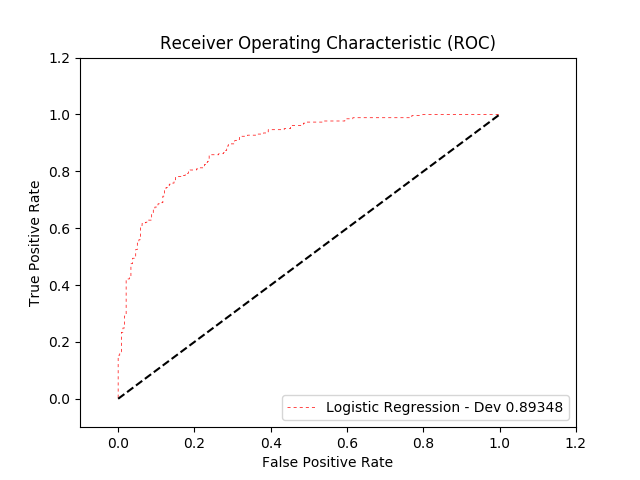
\includegraphics[width=200px, height = 200px]{lr_}
  \caption{AUC for Logistic Regression}
  \label{lr_fig}
\end{figure}

So we see, that we get nearly comparable results with both the Logistic Regression implementations, indicating that the data is linearly separable. We thus move onto more linear models.

\subsection{Support Vector Machine (RBF)}
We tried different regularization parameter. The only hyperparameter tuned was : \textit{$C$} (Slack Penalty). The results are summarized in Table \ref{tab_svm2}. The results in this table are calculated at $C = 0.3$.

\begin{table}[!htb]
 \centering
 \caption{AUC for SVM (rbf)}
 \label{tab_svm2}
\begin{tabular}{ c c c } 
	    \noalign{\smallskip}\hline\noalign{\smallskip}
		Data &   AUC \\
    	   \noalign{\smallskip}\hline\noalign{\smallskip}
		Train & 0.9288767\\
		Dev set & 0.8558008\\
		
  \end{tabular} 
\end{table}

\subsection{Support Vector Machine (Linear)}
We tried different regularization parameter. The only hyperparameter tuned was : \textit{$C$} (Slack Penalty). The results are summarized in Table \ref{tab_svm}.  The results in this table are calculated at $C = 0.3$.

\begin{table}[!htb]
 \centering
 \caption{AUC for SVM (linear)}
 \label{tab_svm}
\begin{tabular}{ c c c } 
	    \noalign{\smallskip}\hline\noalign{\smallskip}
		Data &   AUC \\
    	   \noalign{\smallskip}\hline\noalign{\smallskip}
		Train & 0.8596409\\
		Dev set & 0.8929928\\
			    \noalign{\smallskip}\hline\noalign{\smallskip}
  \end{tabular} 
\end{table}

So we see, that we get nearly different results with different SVM kernel implementations. This is because the data is linearly separable and hence the linear kernel performs so well.

\subsection{Gaussian Na{\"i}ve Bayes}
With Gaussian Na{\"i}ve Bayes we normalize the data using Z-score normalization, as mentioned in the Pre-Processing. The AUC is presented in Table \ref{nb_tab}.

\begin{table}[!htb]
 \centering
 \caption{AUC for Gaussian Na{\"i}ve Bayes}
 \label{nb_tab}
\begin{tabular}{ c c c } 
	    \noalign{\smallskip}\hline\noalign{\smallskip}
		Data & AUC \\
    	   \noalign{\smallskip}\hline\noalign{\smallskip}
		Train &  0.85311513\\
		Dev Set & 0.88468074\\
		\noalign{\smallskip}\hline\noalign{\smallskip}
  \end{tabular} 
\end{table}

\subsection{Neural Networks}
After trying differ linear models, we did some experiments on non-linear model. We trained and tested the data set on Neural Network. Instead of using a python package, we implemented the code for NN. We tuned the \textit{hidden layer} and \textit{learning rate} parameter,  and tried different loss functions - \textit{Sigmoid Loss}, \textit{tanh Loss}. The data for results of NN is provided in Table \ref{tab_nn}.

\begin{table}[!htb]
 \centering
 \caption{AUC for Neural Networks}
 \label{tab_nn}
\begin{tabular}{ c c c } 
	    \noalign{\smallskip}\hline\noalign{\smallskip}
		Data &  AUC \\
    	   \noalign{\smallskip}\hline\noalign{\smallskip}
		Train &  0.742583466799\\
		Dev set &  0.756661659023\\
				\noalign{\smallskip}\hline\noalign{\smallskip}
  \end{tabular} 
\end{table}

Neural Network did not perform well as expected. This is because of the kind of data set we have at hand. The data set is linearly separable hence the traditional methods outperformed the more complex non-linear model. This shows the significance of data set analysis before model selection because the most promising models may behave differently depending on the features of the data set.  

\subsection{XGBoost Classifier}
In this model we used XGBoost classifier to train our model. We tried tuning various parameters \textit{subsample}, \textit{$\eta$}, \textit{colsample\_bytree}, \textit{max\_depth} and \textit{min\_child\_weight}. The best parameters were found to be \textit{$\eta$} : 0.001, \textit{subsample}: 0.3, \textit{colsample\_bytree}: 0.5, \textit{max\_depth}: 3, \textit{min\_child\_weight}: 5. The following table lists some results. 
 
\begin{table}[!htb]
\centering
\caption{AUC for XGBoost}
\label{tab_lr}
\begin{tabular}{ c c c }
                    \noalign{\smallskip}\hline\noalign{\smallskip}
                                Data  & AUC \\
                   \noalign{\smallskip}\hline\noalign{\smallskip}
                                Train & 0.86786\\
                                Dev set  & 0.88758\\                     
  \end{tabular}
\end{table}
 
In figure \ref{xgboost_fig} we represent the AUC for XGBoost, where the area under the ROC curve is 0.88758.
 
\begin{figure}
\centering
  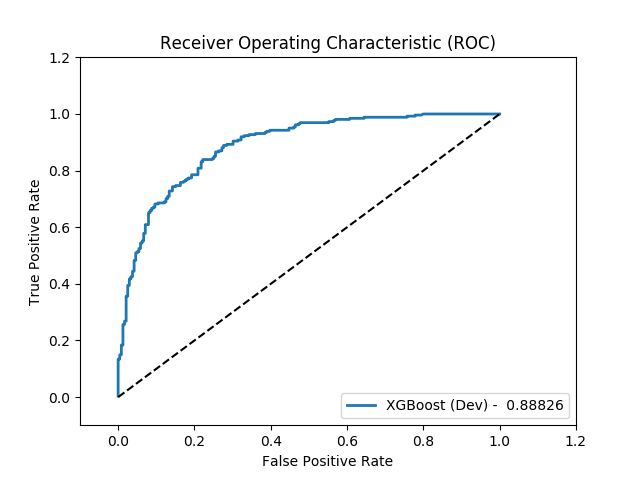
\includegraphics[width=200px, height = 200px]{xgboost_dev}
  \caption{AUC for XGBoost}
  \label{xgboost_fig}
\end{figure}

\section{Conclusions}
Our experiments have shown that the models which rely on linear decision boundaries provide the best results on the given dataset. Among the transforms that we used, logarithimic transform proved to be the most effective because it removed the disparity between the various attributes. From the above experiments we can conclude that the AUC for all our models on the dev set varies between 0.87 - 0.89.
The following table provides a summary of AUC scores on Test Dataset for our submissions made on Kaggle website. We present the results of the best values of the models described above that we submitted. All the results presented here were the ones in which we used Feature selection, as well as did Z-Score \& Log normalization of the data.
\begin{table}[!htb]
\centering
\caption{AUC scores for Test Dataset (As per Kaggle Evaluation)}
\label{tab_lr}
\begin{tabular}{ c c c }
 \noalign{\smallskip}\hline\noalign{\smallskip}
   Model  & AUC \\
 \noalign{\smallskip}\hline\noalign{\smallskip}
 Logistic Regression & 0.86065\\
 XgBoost & 0.86168\\
 Gaussian Na{\"i}ve Bayes & 0.84009\\
 Neural Nets & <Harsh>\\
 SVM & <Harsh> \\
 \end{tabular}
\end{table}

From the table we see that XgBoost performs best since it is an emsemble of several weak classifiers. Followed by XgBoost is Logistic regression. This shows that the data was indeed linearly separable. We also learned about doing an analysis of the dataset, as through our analysis we figured out how the dataset was linearly separable and hence we were able to apply the traditional models instead of the complex models.
Future works on this problem could involve application of PCA to further select combinations of best attributes in order to drive better results.

% (used to reserve space for the reference number labels box)
\begin{thebibliography}{1}
\bibitem{kaggle}
A website for data science competitions. https://www.kaggle.com/
\bibitem{kaggle2}
Influencers in Social Networks : https://www.kaggle.com/c/predict-who-is-more-influential-in-a-social-network
\bibitem{roc}
https://en.wikipedia.org/wiki/Receiver\_operating\_characteristic
\bibitem{svm}
Sci-kit learn Support Vector Machines : http://scikit-learn.org/stable/modules/generated/sklearn.svm.SVC.html
\bibitem{gnb}
Sci-kit learn Gaussian Na{\"i}ve Bayes : http://scikit-learn.org/stable/modules/generated/sklearn.naive\_bayes.GaussianNB.html

\bibitem{xgboost}
XGBoost Library : https://pypi.python.org/pypi/xgboost/
\end{thebibliography}

% that's all folks
\end{document}
